\documentclass[../main.tex]{subfiles}
\graphicspath{{\subfix{images/}}}
\setlength{\parskip}{1.5em}

\begin{document}
    \textbf{Example 2:} Given two different colours of beads, how many unique bracelets of size 8 can you make?
    
    The first step in solving this problem is determining the order of the group acting on the bracelet. We will use the graph on 8 vertices below to represent the bracelet because its vertices are connected in the same way as a bracelet with 8 beads.

    \begin{center}
    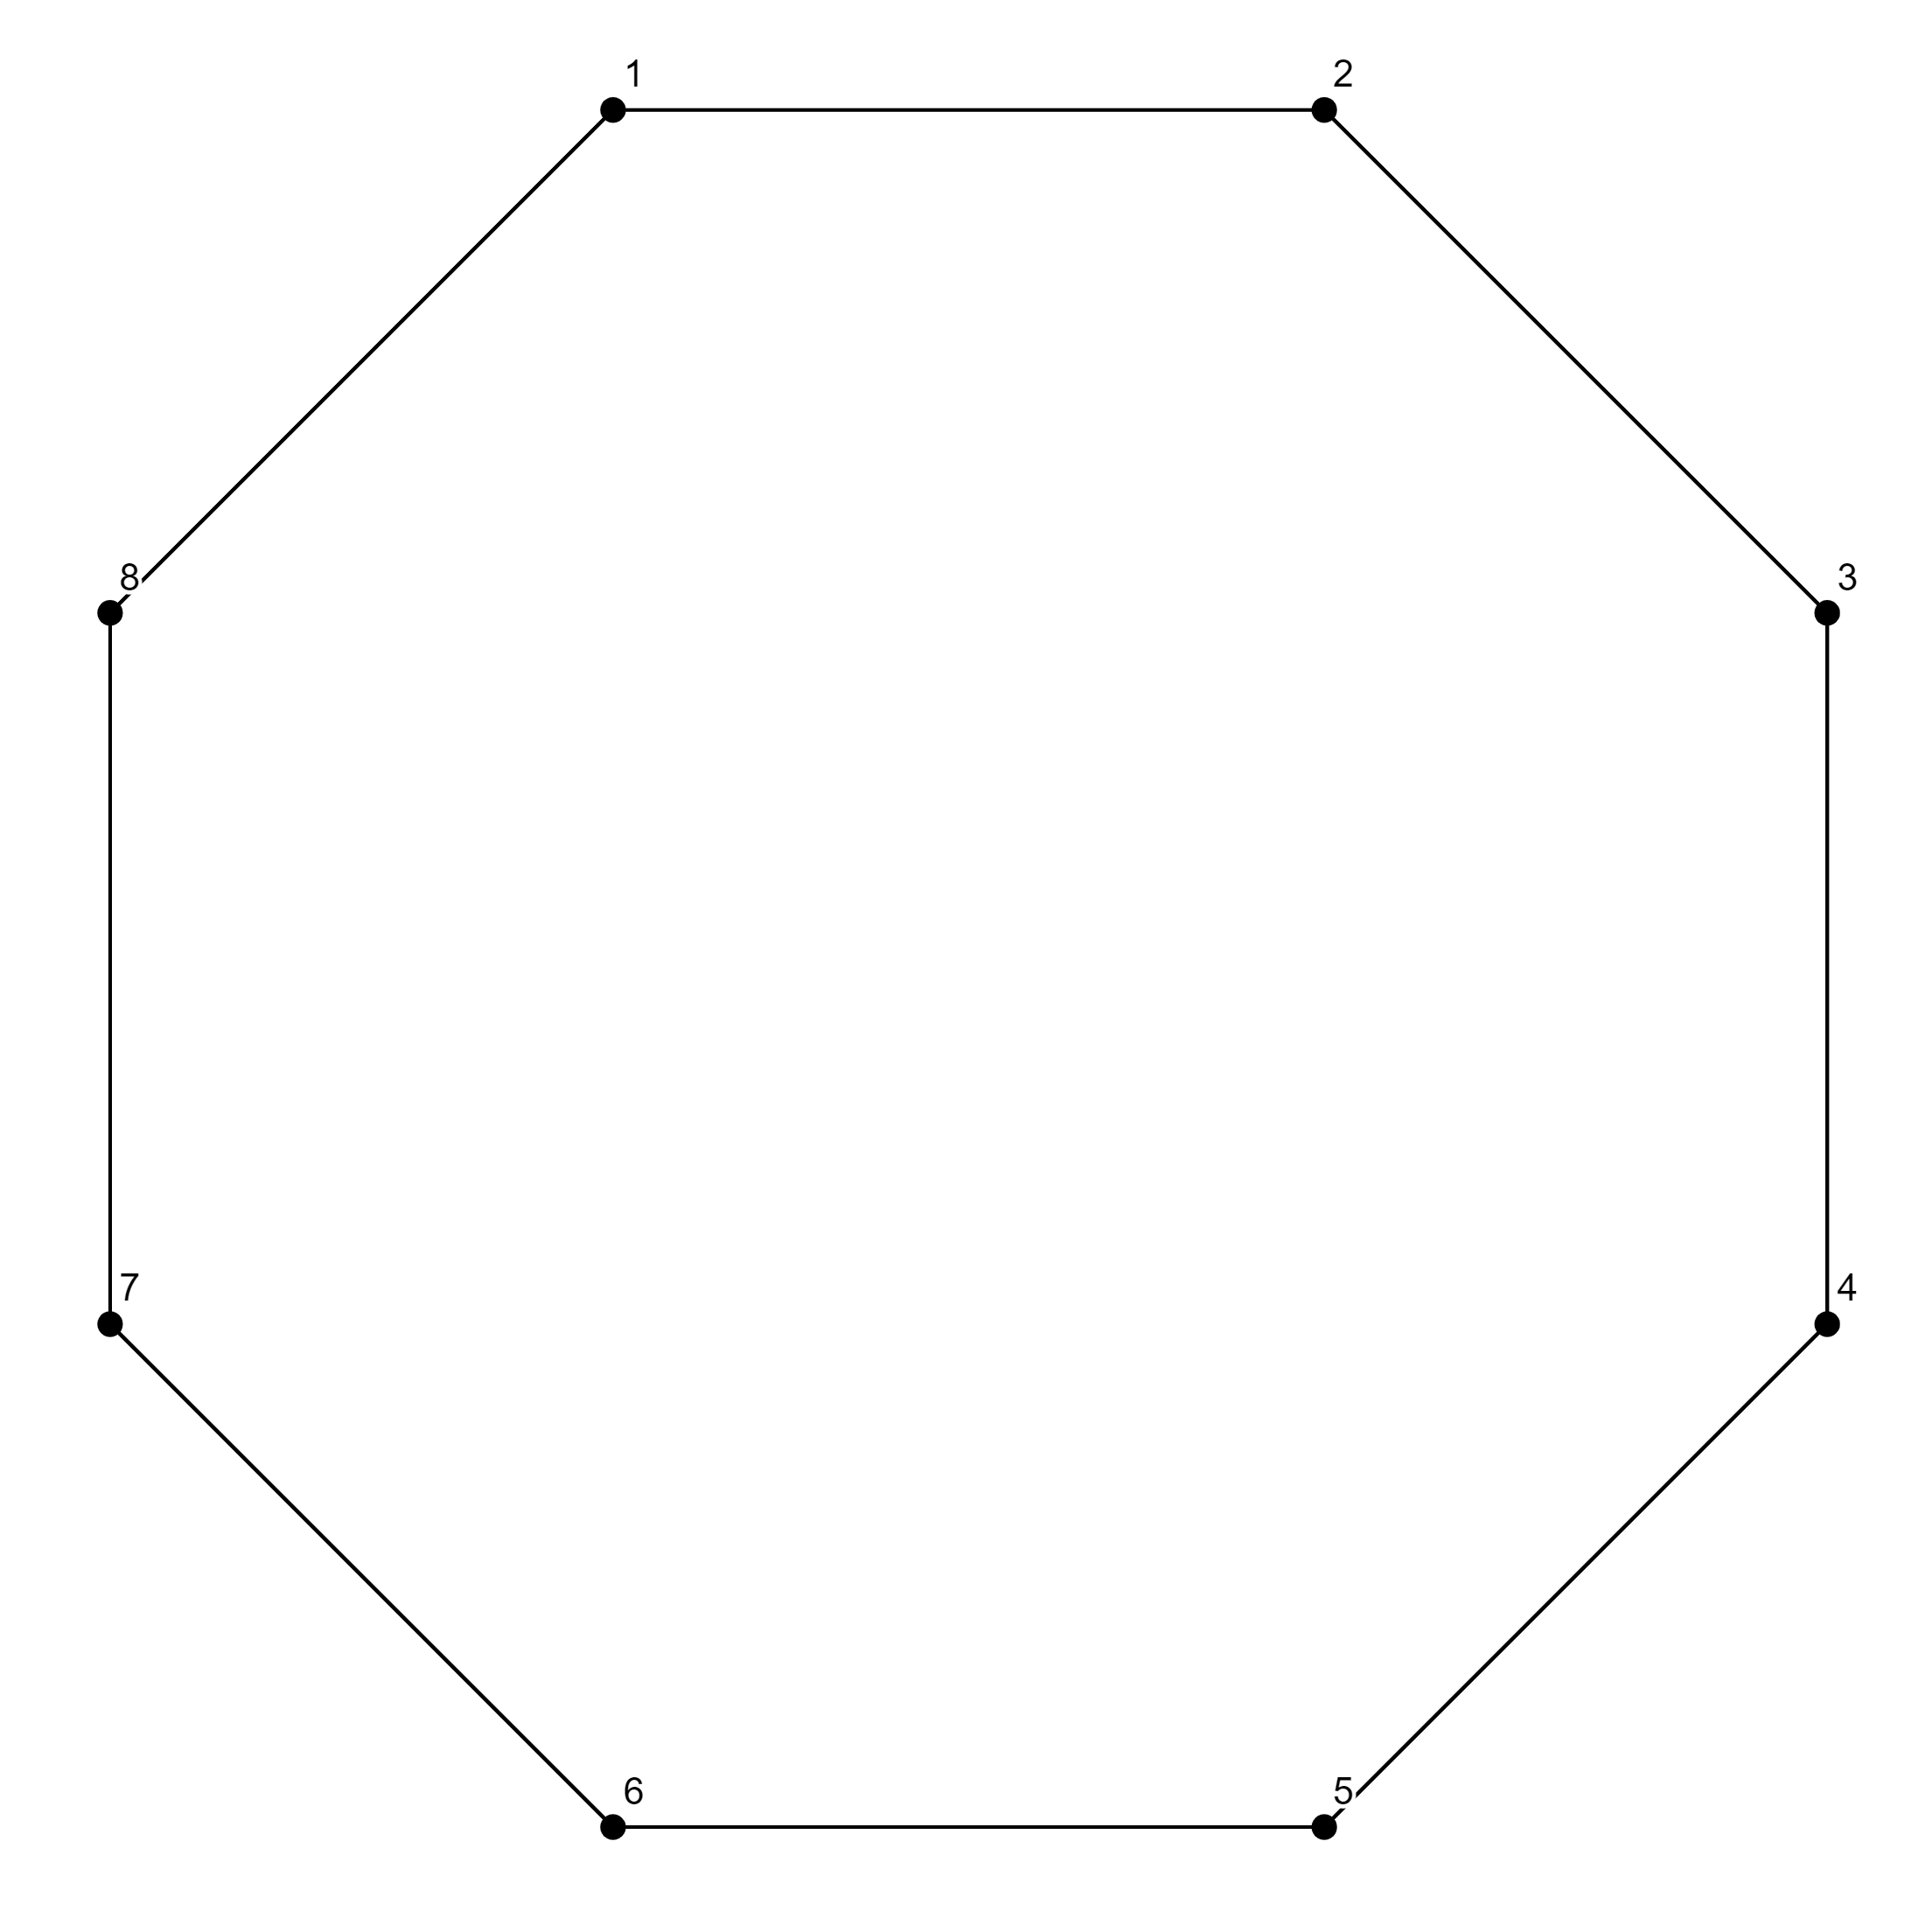
\includegraphics[width=80mm]{images/D8.png}   
    \end{center}

    Let $X$ be the set of all possible bracelets with two colours of size 8, and let $G$ be the group of symmetries that act on $X$. The first thing we must do is calculate the order of $G$ using the orbit-stabilizer theorem.

    Since $G$ is the group of symmetries; rather than acting on the set of all possible colouring's we can instead act on the set of vertices which we will denote $Y$. Looking at our diagram its clear that any vertex $y \in Y$ can be rotated to any other vertex, and the only two symmetries that fix $y$ are the identity element and a reflection on the line through $y$ and its opposite vertex. So it follows that $Orb(y) = 8$ and $G_y = 2$, and as a corollary the elements of $G$ can be generated by a rotation and a reflection. Applying the orbit-stabilizer theorem we find that $\lvert G \rvert = 8 \cdot 2 = 16$. 

    Next we need to find $X^g$ for each $g \in G$, to specify actions in $G$ we will write them in terms of a $\frac{1}{8}$th clockwise rotation which we will call $r$ and a reflection on the line in the diagram below which we will call $t$.

    \begin{center}
    \includegraphics[width=85mm]{images/D8_sym.png}   
    \end{center}

    Recall that a group $G$ acting on $X$ is a group homomorphism from $G$ to the set of possible permutations on $X$, so it follows that $\phi(g) \in S(X)$. This means that $r$ and $t$ can be expressed as the following permutations of $X$.
    
    \begin{align*}
        r &= (1 \;2 \;3 \;4 \;5 \;6 \;7 \;8) \\
        t &= (1 \;2)(3 \;8)(4 \;7)(5 \;6)
    \end{align*}

    By expressing a group action in terms of permutation cycles, the elements of $X$ that are fixed by the group action become much more clear.

    Take for example $X^r$, we can see that $r$ takes the first vertex to the second vertex, this means that vertex 1 and 2 must be the same colour. Continuing on we see that $r$ takes the second vertex to the third vertex, and so forth. Eventually we find that every vertex must have the same colour and since there are only 2 colours this means that $\lvert X^r \rvert = 2$. 

    Investigating further we find that if $x \in X^g$ then $x$ must be coloured in such a way that each cycle in $\phi(g)$ contains vertices of the same colour. Now lets calculate the cycles for the elements in $G$.
    \hfill
    \begin{center}
        \begin{tabular}{ |p{1cm}|p{5cm}|p{1cm}||p{1cm}|p{5cm}|p{1cm}|  }
            \hline
            $\mathbf{g}$ & \textbf{Cycle} & $\lvert \mathbf{X^g} \rvert$ &$\mathbf{g}$ & \textbf{Cycle} & $\lvert \mathbf{X^g} \rvert$ \\
            \hline
            \hline
            $e$     & $(1)(2)(3)(4)(5)(6)(7)(8)$ & $2^8$    &                $t$     & $(1\;2)(3\;8)(4\;7)(5\;6)$ & $2^4$    \\
            \hline
            $r$     & $(1\;2\;3\;4\;5\;6\;7\;8)$ & $2^1$    &                $rt$    & $(1)(5)(2\;8)(3\;7)(4\;6)$ & $2^5$    \\
            \hline
            $r^2$   & $(1\;3\;5\;7)(2\;4\;6\;8)$ & $2^2$    &                $r^2t$  & $(1\;8)(2\;7)(3\;6)(4\;5)$ & $2^4$    \\
            \hline
            $r^3$   & $(1\;4\;7\;2\;5\;8\;3\;6)$ & $2^1$    &                $r^3t$  & $(4)(8)(1\;7)(2\;6)(3\;5)$ & $2^5$    \\
            \hline
            $r^4$   & $(1\;5)(2\;6)(3\;7)(4\;8)$ & $2^4$    &                $r^4t$  & $(1\;6)(2\;5)(3\;4)(7\;8)$ & $2^4$    \\
            \hline
            $r^5$   & $(1\;6\;3\;8\;5\;2\;7\;4)$ & $2^1$    &                $r^5t$  & $(7)(3)(1\;5)(2\;4)(6\;8)$ & $2^5$    \\
            \hline
            $r^6$   & $(1\;7\;5\;3)(2\;8\;6\;4)$ & $2^2$    &                $r^6t$  & $(1\;4)(2\;3)(5\;8)(6\;7)$ & $2^4$    \\
            \hline
            $r^7$   & $(1\;8\;7\;6\;5\;4\;3\;2)$ & $2^1$    &                $r^7t$  & $(2)(6)(1\;3)(4\;8)(5\;7)$ & $2^5$    \\
            \hline
        \end{tabular}
    \end{center}
    \hfill

    Plugging the values from the table below into Burnside's lemma we get the following equation
    \begin{equation*}
        \begin{split}
            \lvert X / G \rvert & = \frac{2^8 + 4 \cdot 2^1 + 2 \cdot 2^2 + 5 \cdot 2^4 +4 \cdot 2^5}{16} \\
            & = 30
        \end{split}
    \end{equation*}
    
    So with 8 beads of two colours there are a 30 possible bracelets that are unique.
    
    \textbf{Example 3:} What if in the previous example we had 3 colours rather than 2 how many unique bracelets could you make?
    
    In this problem the only difference is that the vertices in each cycle can be 3 three possible colours rather than 2. So the formula for the number of orbits is
    \begin{equation*}
        \begin{split}
            \lvert X / G \rvert & = \frac{3^8 + 4 \cdot 3^1 + 2 \cdot 3^2 + 5 \cdot 3^4 +4 \cdot 3^5}{16} \\
            & = 498
        \end{split}
    \end{equation*}
    
    \textbf{Example 4:} Given two different colours of beads, how many unique necklaces of size 15 can you make?
    
    This problem is similar to the previous problems, the only difference is that necklaces aren't symmetric under reflection. This problem is much easier to solve, especially if the number of beads is prime but we will get to that in the next example. 
    
    Since the necklace only has 2D rotational symmetry and 15 vertices, by inspection we can determine that $\lvert G \rvert = 15$ and $G =\langle r \rangle$ where $r$ is a $\frac{1}{15}$th rotation.
    
    Because the group $G$ is generated by a single element it must be a cyclic group, an isomorphic to $\mathbb{Z}_{15}$. Note that 3 and 5 are prime divisors of $\lvert G \rvert$, which means that $G$ must also have cyclic subgroups of prime order. 
    
    Suppose $G$ is acting on a regular polygon with a set $X$ of 15 vertices.
    
    For any given rotation $r^n$ we know that if $n$ is co-prime to 15 then the LCM$(n, 15) = n \cdot 15$ which means that $r^n$ is only equal to the identity after 15 permutations and must have a cycle of 15. This is true for $ n \in \{1,2,4,7,8,11,13,14\}$.
    
    Now if $n \in \{3,6,9,12\}$ then $r^n$ contains three 5-cycles. As you can see in the figures below $r^3$ and $r^6$  
    
    \begin{figure*}[!htb]
        \captionsetup[subfigure]{labelformat=empty}
            \centering
            \subfloat[$r^3$]{{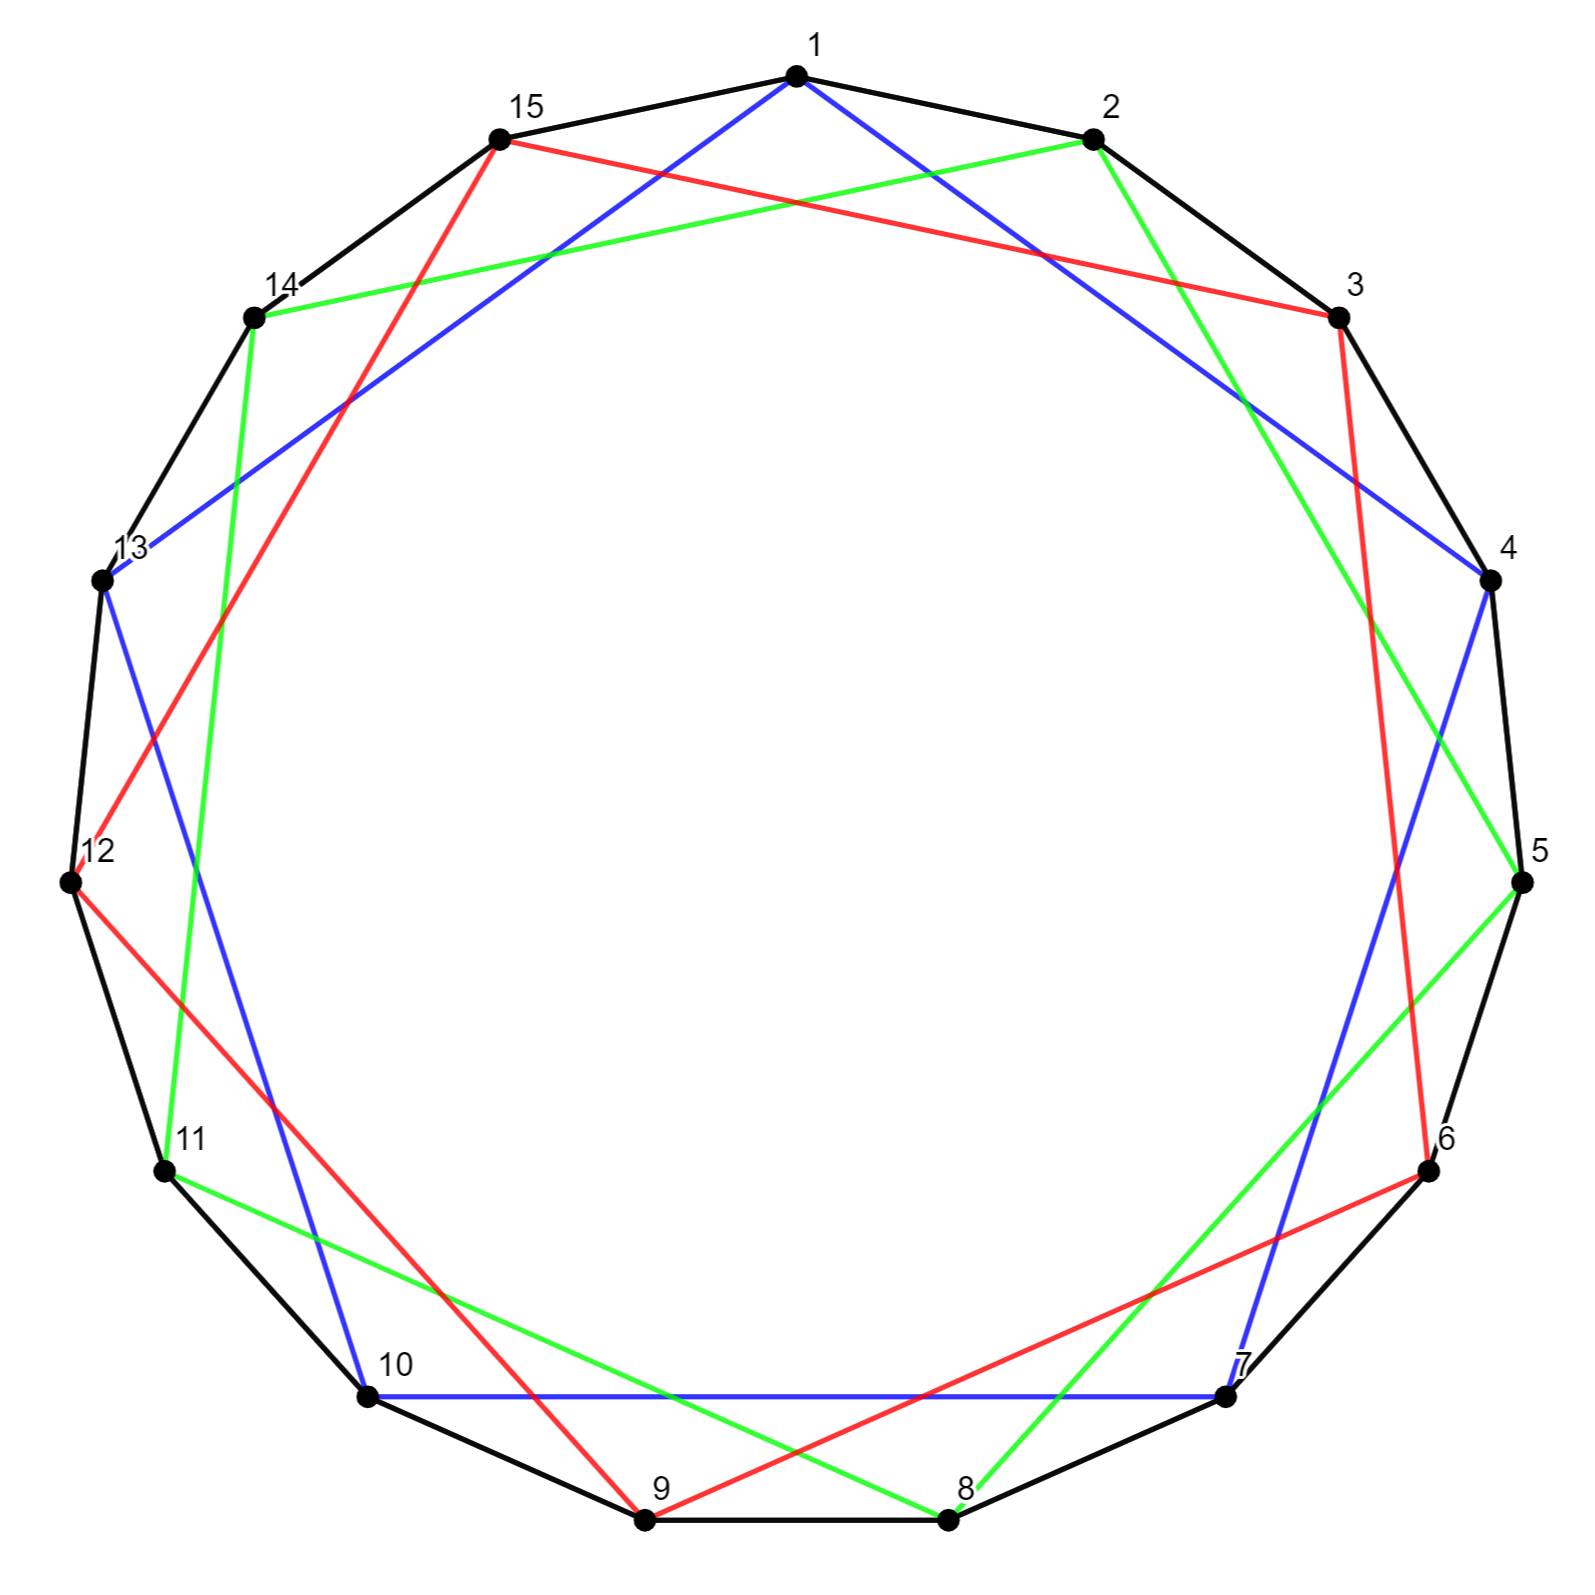
\includegraphics[width=7.5cm]{images/C15-3.png} }}
            \subfloat[$r^6$]{{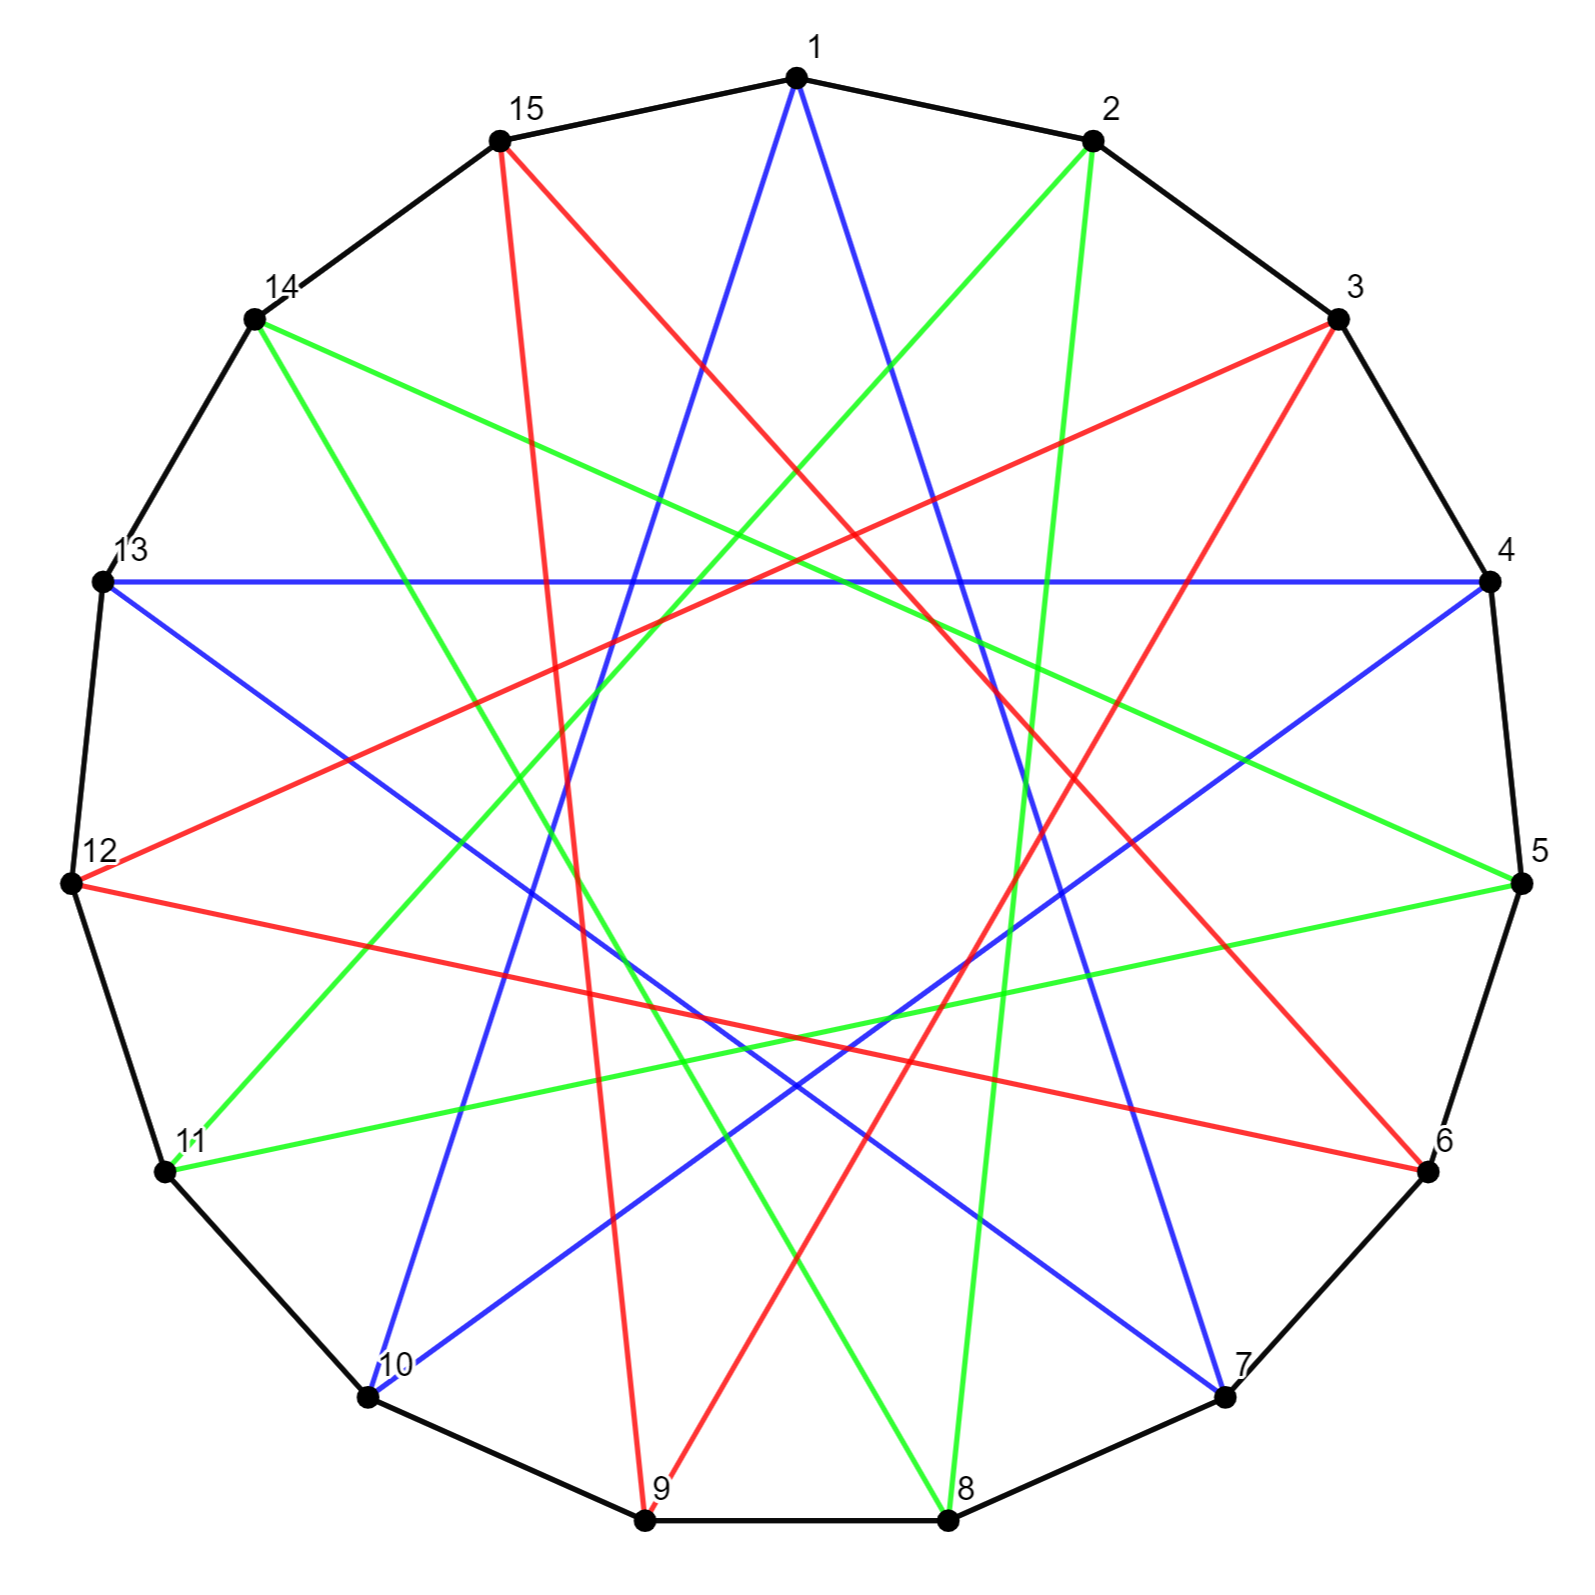
\includegraphics[width=7.5cm]{images/C15-6.png} }}
            \label{steady_state}
    \end{figure*}
    This isn't much of a surprise as $3 \cdot 5 = 6 \cdot 5 = 9 \cdot 5 = 12 \cdot 5 = 0$ under addition mod 15.
    
    Following the same logic as before, if $n \in \{5, 10\}$ then $r^n$ contains five 3-cycles. 
    
    Making sure we don't forget the identity $e$ with $15$ fixed points were ready to move on. 
    
    For two different colours of beads, we end up with 2 choices per cycle in each symmetry of $G$. Plugging into Burnside's lemma we get
    \begin{align*}
        \lvert X / G \rvert & = \frac{8 \cdot 2^1 + 4 \cdot 2^3 + 2 \cdot 2^5 + 1 \cdot 2^{15}}{15} \\
        & = 2192
    \end{align*}
    
    \textbf{Example 4:} Given two different colours of beads, how many unique necklaces of size 31 can you make?
    
    Using the same logic as the previous question we come to the conclusion that $G$ is a cyclic group acting on a set of 31 vertices $X$. However in this case we find that $\lvert G \rvert = 31$ which is prime. This means that $G$ has no non-trivial subgroups and as a consequence every possible permutation in $G$ aside from the identity has a cycle of size 31. This leaves us with the equation
        \begin{align*}
        \lvert X / G \rvert & = \frac{30 \cdot 2^1 + 1 \cdot 2^{31}}{31} \\
        & = 69273668
    \end{align*}
    
    
    
    

    
    
    
    
    
    
    
    
\end{document}
